\documentclass[11pt,border=2pt]{standalone}
\usepackage{amsmath,amssymb}
\usepackage{xcolor}
\usepackage{tikz}
\usepackage{pgfplots}
\pgfplotsset{compat=1.18}
\usetikzlibrary{calc,arrows,positioning,fit,backgrounds,decorations.pathreplacing,patterns}
\definecolor{cElem}{RGB}{40,80,140}
\definecolor{cTrg}{RGB}{190,40,40}
\definecolor{cCell}{RGB}{225,238,248}
\definecolor{cAcc}{RGB}{240,200,120}
\definecolor{cGrey}{RGB}{120,120,120}
\definecolor{cVec}{RGB}{110,55,150}
\begin{document}
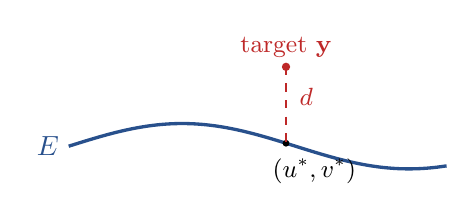
\begin{tikzpicture}[scale=2.4]
  \draw[cElem,very thick] plot[smooth,domain=0:2,samples=40] (\x,{0.12*sin(150*\x)});
  \node[cElem,left] at (0,0) {$E$};
  \fill[cTrg] (1.15,0.42) circle (0.022) node[above,cTrg,font=\small] {target $\mathbf{y}$};
  \fill[black] (1.15,{0.12*sin(150*1.15)}) circle (0.018);
  \node[below,font=\small] at (1.30,{0.12*sin(150*1.15)-0.03}) {$(u^\ast,v^\ast)$};
  \draw[dashed,cTrg] (1.15,0.42) -- (1.15,{0.12*sin(150*1.15)});
  \node[cTrg,right,font=\small] at (1.17,0.26) {$d$};
\end{tikzpicture}
\end{document}
